\usetikzlibrary{arrows.meta,calc,shapes}
\providecommand{\computer}{%
    
\includegraphics[width=1cm,alt=computer]{../common/Noun_project_216.pdf}
}
\providecommand{\switch}{%
    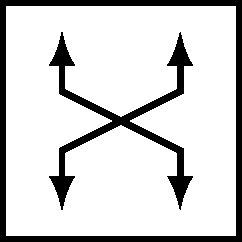
\includegraphics[width=0.9cm,alt=switch]{../common/fig-switch.pdf}
}
\providecommand{\router}{%
    
\includegraphics[width=0.9cm,alt=router]{../common/fig-router.pdf}
}

\begin{frame}[fragile]\frametitle{exercise} % FIXME: text description
\myalttext{
\begin{tikzpicture}
\tikzset{
    computer/.style={inner sep=0mm,outer sep=0mm,execute at begin node={\computer}},
    switch/.style={inner sep=0mm,outer sep=0mm,execute at begin node={\switch}},
    router/.style={inner sep=0mm,outer sep=-1mm,execute at begin node={\router},circle},
    connect/.style={draw,very thick,Latex-Latex},
    connect big/.style={draw,ultra thick,Latex-Latex},
    other/.style={opacity=0.5},
}
\node[computer,label={north:video stream server}] (server) at (0, 0) {};
\node[computer,label={south:user C}] (C) at (6, 0) {};
\node[computer,label={south:user D}] (D) at (6, -2) {};
\node[computer,label={south:user A}] (A) at (-6, 0) {};
\node[computer,label={south:user B}] (B) at (-6, -2) {};
\node[computer,other] (other1) at (-4.3, 0) {};
\node[computer,other] (other2) at (4.5, 0.5) {};
\node[switch] (other3) at (-2,-1) {};
\node[computer,other] (other4) at (-2.7, 0.2) {};
\node[switch] (s1) at (-3, -2) {};
\node[router] (s2) at (0, -2) {};
\node[switch] (s3) at (2, -1) {};
\node[switch] (s4) at (4, -2) {};
\foreach \x/\y in {A/s1,B/s1,s1/s2,server/s2,s2/s3,s3/s4,s4/D,s3/C,s1/other1,s3/other2,s2/other3,other3.west/other4} {
    \draw[connect] (\x) -- (\y);
}
\end{tikzpicture}
}{video stream server <-> circle <-> {square <-> {user C, square <-> used D}, square <-> unlabeled computer, square <-> {user A, user B}}}
    \begin{itemize}
    \item if each of users A--D are receiving (potentially different) video 
    and audio from the video streaming server, then\ldots
        \begin{itemize}
        \item how many flows?
        \item how many nodes are involved?
        \item how many switches/routers?
        \end{itemize}
    \end{itemize}
\end{frame}

